\documentclass[xcolor=pdftex,dvipsnames,table,mathserif,aspectratio=169]{beamer}
\usetheme{default}
\usetheme{metropolis}
\usepackage{minted}
\usepackage{mathtools}
\setbeamersize{text margin left=.3in,text margin right=.3in} 

\usepackage[english]{babel}
\usepackage{pgf,pgfarrows,pgfnodes,pgfautomata,pgfheaps}
\usepackage{amsmath,amssymb,setspace,centernot}
\usepackage[latin1]{inputenc}
\usepackage{pgf,tikz}
\usepackage[T1]{fontenc}
\usepackage{relsize}
\usepackage{pdfpages}
\usepackage[absolute,overlay]{textpos} 


\DeclareMathOperator*{\argmax}{arg\,max}
\DeclareMathOperator*{\argmin}{arg\,min}

\newcommand{\X}{\mathtt{X}}
\newcommand{\Y}{\mathtt{Y}}

%\newcommand{\R}{\mathbb{R}}
%\newcommand{\E}{\mathbb{E}}
%\newcommand{\V}{\mathbb{V}}
\newcommand{\p}{\mathbb{P}}
\newcommand*\df{\mathop{}\!\mathrm{d}}
\newcommand{\del}{\partial}


% imports
\usepackage{xargs}
\usepackage{xpatch}
\usepackage{etoolbox}
\usepackage{pdflscape}
\usepackage{booktabs}
\usepackage{threeparttable}
\usepackage[skip=0.2\baselineskip]{caption}

% command for inputting raw latex
\makeatletter
\newcommand\primitiveinput[1]{\@@input #1 }
\makeatother

% common table command
\newcommandx{\tablecontent}[4]{
    \begin{threeparttable}[!ht]
        \centering
        \caption{#3}
        \vspace{-1em}
        \footnotesize
        \begin{tabular}{#1}
            \primitiveinput{../tables/#2.tex}
        \end{tabular}
        \vspace{-0.2em}
        \begin{tablenotes}[flushleft]
            #4
        \end{tablenotes}
    \end{threeparttable}
}




% \usepackage{slashbox}
\title{ Advanced Panel Data:\\
Interpreting FE?}
\author{Chris Conlon }
\institute{NYU Stern }


\newcommand{\norm}[1]{\left\lVert#1\right\rVert}
\newcommand{\R}{\mathbb{R}}
\newcommand{\E}{\mathbb{E}}
\newcommand{\V}{\mathbb{V}}
\newcommand{\ol}{\overline}
%\newcommand{\ul}{\underline}
\newcommand{\pp}{{\prime \prime}}
\newcommand{\ppp}{{\prime \prime \prime}}
\newcommand{\policy}{\gamma}


\newcommand{\fp}{\frame[plain]}

\date{\today}

\begin{document}
\maketitle

\section*{Causal FE}

\begin{frame}
\frametitle{Recall the FE Assumptions}
\begin{eqnarray*}
y_{it} =  x_{it}'\beta + \eta_i + \varepsilon_{it}
\end{eqnarray*}
\begin{itemize}
\item $\eta_i$ is a \alert{fixed effect}.
\item To estimate everything consistently, we need $E[ \varepsilon_{it} | x_{it}, \eta_i]=0$
\item Mostly this is not true. Instead usually treat $\eta_i$ as a \alert{control variable} or \alert{nuisance parameter}.
\begin{itemize}
\item A nuisance parameter is one that we estimate but don't care about interpreting.
\item If we only care about $\beta$ then $\eta_i$ is a nuisance parameter.
\end{itemize}
\item With a control or nuisance parameter we only require that $E[ \varepsilon_{it} | \eta_{i}]=E[ \varepsilon_{it} | x_{it}, \eta_i]$ \alert{conditional mean independence}.
\end{itemize}
\end{frame}

\begin{frame}
\frametitle{Recall the FE Assumptions}
\begin{eqnarray*}
y_{it} =  x_{it}'\beta + \eta_i + \varepsilon_{it}
\end{eqnarray*}
\begin{itemize}
\item $\eta_i$ is a \alert{fixed effect}.
\item To estimate everything consistently, we need $E[ \varepsilon_{it} | x_{it}, \eta_i]=0$
\item Mostly this is not true. Instead usually treat $\eta_i$ as a \alert{control variable} or \alert{nuisance parameter}.
\begin{itemize}
\item A nuisance parameter is one that we estimate but don't care about interpreting.
\item If we only care about $\beta$ then $\eta_i$ is a nuisance parameter.
\end{itemize}
\item With a control or nuisance parameter we only require that $E[ \varepsilon_{it} | \eta_{i}]=E[ \varepsilon_{it} | x_{it}, \eta_i]$ \alert{conditional mean independence}.
\item Once we condition on $\eta_i$ it is as if $\varepsilon_{it}$ and $x_{it}$ are uncorrelated.
\end{itemize}
\end{frame}


\begin{frame}{Causal FE}
\begin{itemize}
\item We can get away with conditional mean independence if we don't care about $\eta_i$.
\item But suppose that we care about $\widehat{\eta}_i$?
\begin{itemize}
\item Teacher FE
\item Physician/Hospital FE
\item Location/County FE
\item Suppose we take someone from the $10th$ percentile and move them to the $90th$ percentile
\end{itemize}
\end{itemize}
\end{frame}


\begin{frame}{Causal FE}
\begin{itemize}
\item Now we have to really believe $E[ \varepsilon_{it} | x_{it}, \eta_i]=0$
\item We should worry about the conventional \alert{omitted variable bias} problem.
\item Suppose there exists a variable $w_{it}$ so that:
\begin{eqnarray*}
y_{it} =  x_{it}'\beta +  w_{it}'\gamma + \eta_i + \varepsilon_{it}
\end{eqnarray*}
\item Recall the conditions for OVB
\begin{itemize}
\item $w_{it}$ is correlated with $x_{it}$
\item $w_{it}$ is a determinant of $y_{it}$
\end{itemize}
\item New one:  $w_{it}$ is correlated with $\eta_i$
\begin{itemize}
\item This is easy to satisfy!
\item $w_{it}$ needs to be uncorrelated with anything about the individual $i$.
\end{itemize}
\end{itemize}
\end{frame}



\begin{frame}{Example: Test Scores}
\begin{itemize}
\item Students $s$, Teachers $t$
\item Want to measure effect of \alert{Teachers} on \alert{Test Scores}
\begin{eqnarray*}
TestScore_{st} = \beta x_s +\gamma w_t+  \eta_{i} + \varepsilon_{st}
\end{eqnarray*}
\item We observe some features of students but not all of them (parent's education, household income, language spoken at home).
\item We also observe some school specific variables $w_t$ but not all of them (district spending per pupil, \% free lunch, etc.).
\item But we don't observe other things (jackhammering outside the classroom, which students have disruptive home lives,etc.).
\begin{itemize}
\item If the mean of those things varies across teachers $\rightarrow$ we are screwed!
\item Can't get an accurate estimate of $\eta_i$.
\end{itemize}
\end{itemize}
\end{frame}


\begin{frame}{Example: Test Scores}
We need a better design:
\begin{itemize}
\item We probably need random assignment of students to teachers.
\item Ideally we would be able to control for student and school unobservables.
\item Might want to see many students match with many teachers.
\end{itemize}
\end{frame}

\begin{frame}{Healthcare Exceptionalism: Static Reallocation}
Is \alert{quality} (or productivity) correlated with \alert{market share}?
\begin{align*}
\ln \left(N_{h}\right)=\beta_{0}^{s}+\beta_{1}^{s} q_{h}+\gamma_{M}^{S}+\varepsilon_{h}^{s}
\end{align*}
\begin{itemize}
\item $N_h$ measures market size for hospital $h$
\item $\gamma_M^s$ are market FE
\item $q_h$ is measure of hospital quality
\item Goal: Is $\beta_1^s>0$ or not. $\beta_1^s<0$ is usually only Soviet countries or 1970's steel.
\item $\beta_1^s>0$ means allocation towards productive firms (or just returns to scale?)
\end{itemize}
\end{frame}

\begin{frame}{Healthcare Exceptionalism: Dynamic Reallocation}
\begin{align*}
\Delta_{h}&=\beta_{0}^{d}+\beta_{1}^{d} q_{h}+\gamma_{M}^{d}+\varepsilon_{h}^{d}\\
\Delta_{h}&=\frac{N_{h, 2010}-N_{h, 2008}}{\frac{1}{2}\left(N_{h, 2010}+N_{h, 2008}\right)}
\end{align*}
\begin{itemize}
\item $\beta_1^d>0$ means growth towards productive firms (not just returns to scale)
\item Same idea but now we capture \alert{dynamics}.
\item Patients may still be attracted to \alert{unobservables correlated with quality}.
\end{itemize}
\end{frame}


\begin{frame}{Healthcare Exceptionalism}
\begin{center}
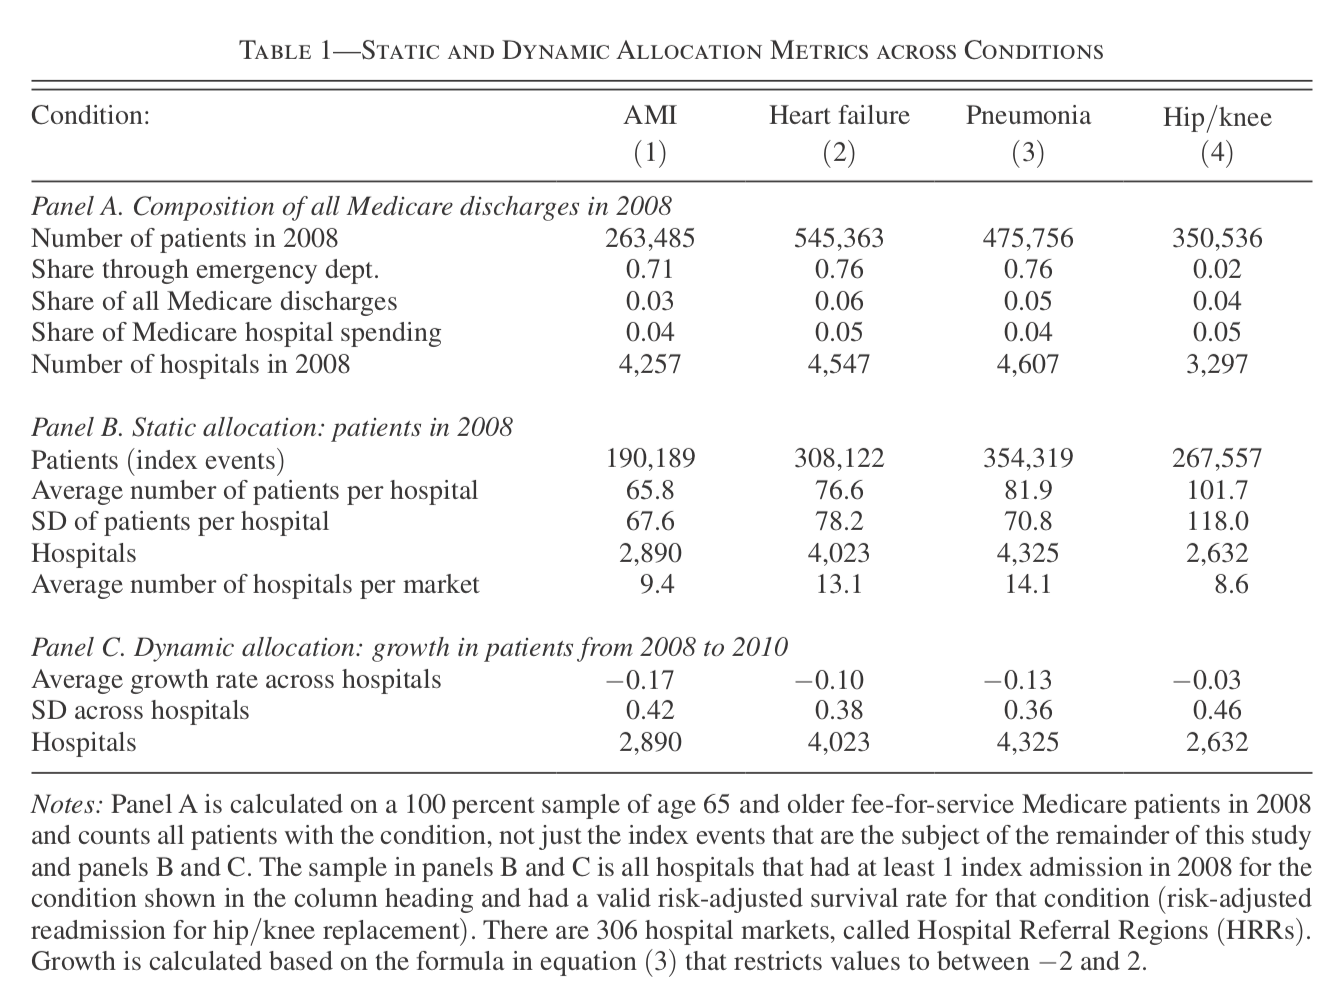
\includegraphics[width=4in]{./resources/hc1.png}
\end{center}
\end{frame}

\begin{frame}{Healthcare Exceptionalism}
\begin{center}
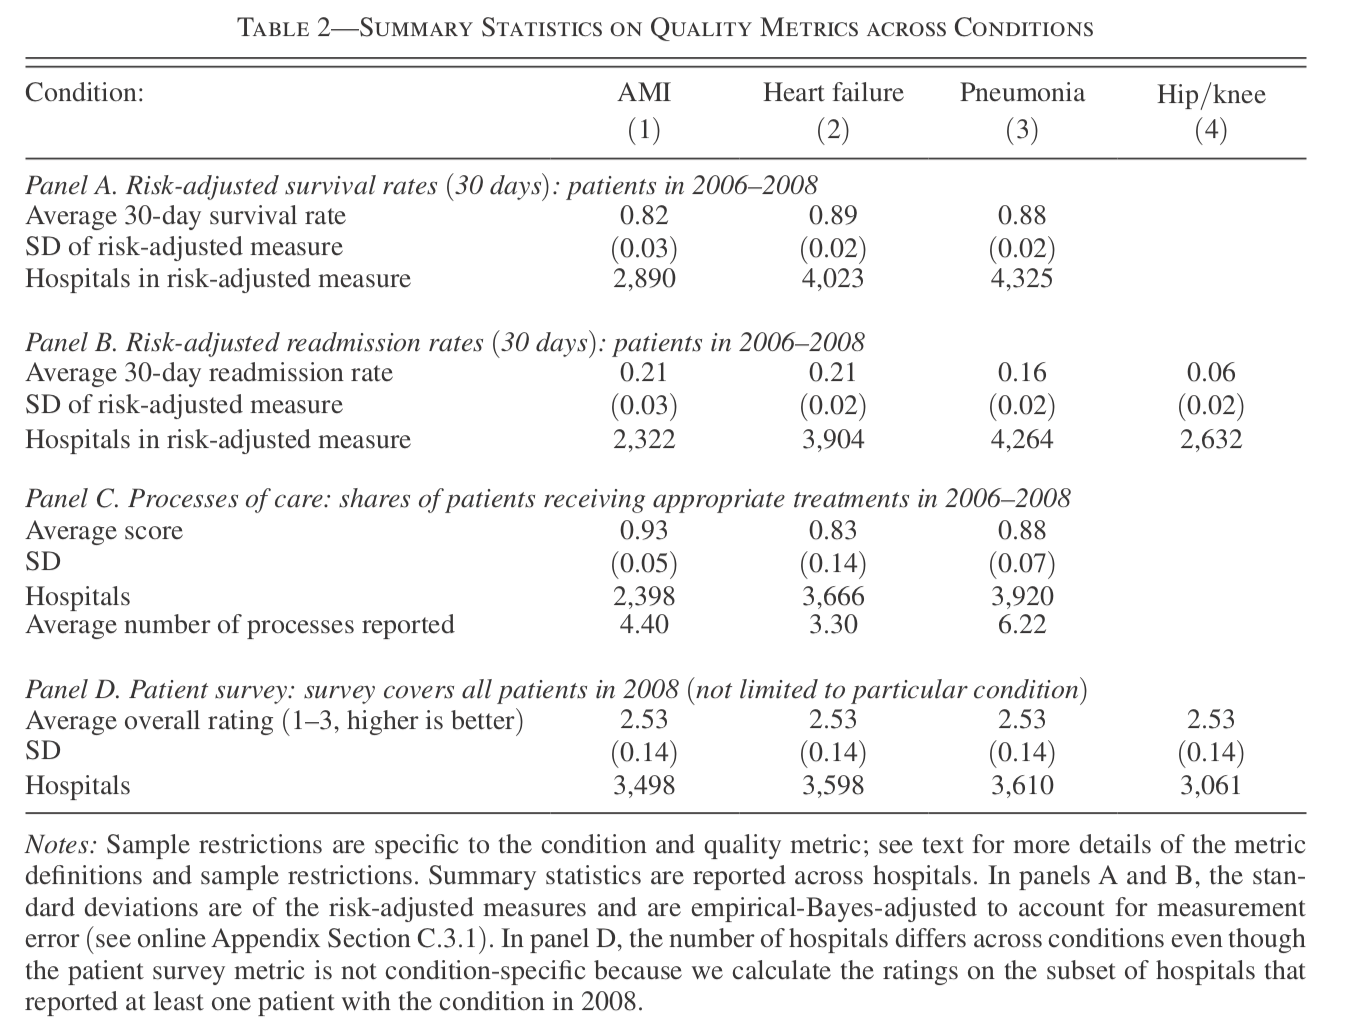
\includegraphics[width=4in]{./resources/hc2.png}
\end{center}
\end{frame}

\begin{frame}{Healthcare Exceptionalism}
\begin{center}
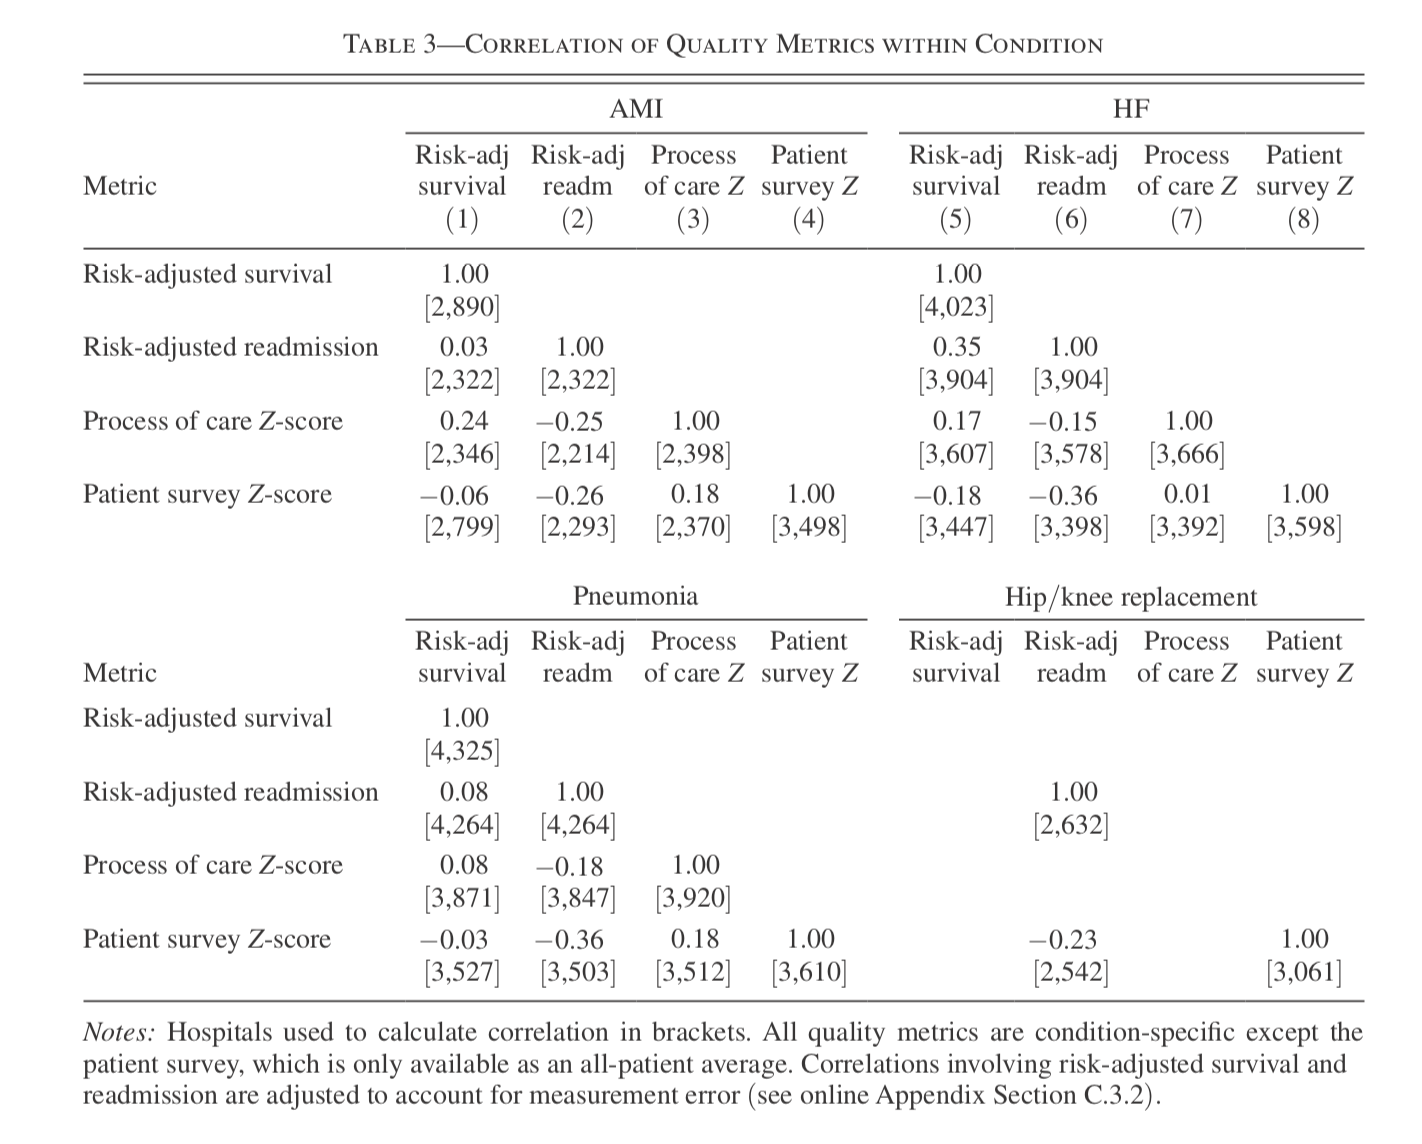
\includegraphics[width=4in]{./resources/hc3.png}
\end{center}
\end{frame}

\begin{frame}{Healthcare Exceptionalism}
\begin{center}
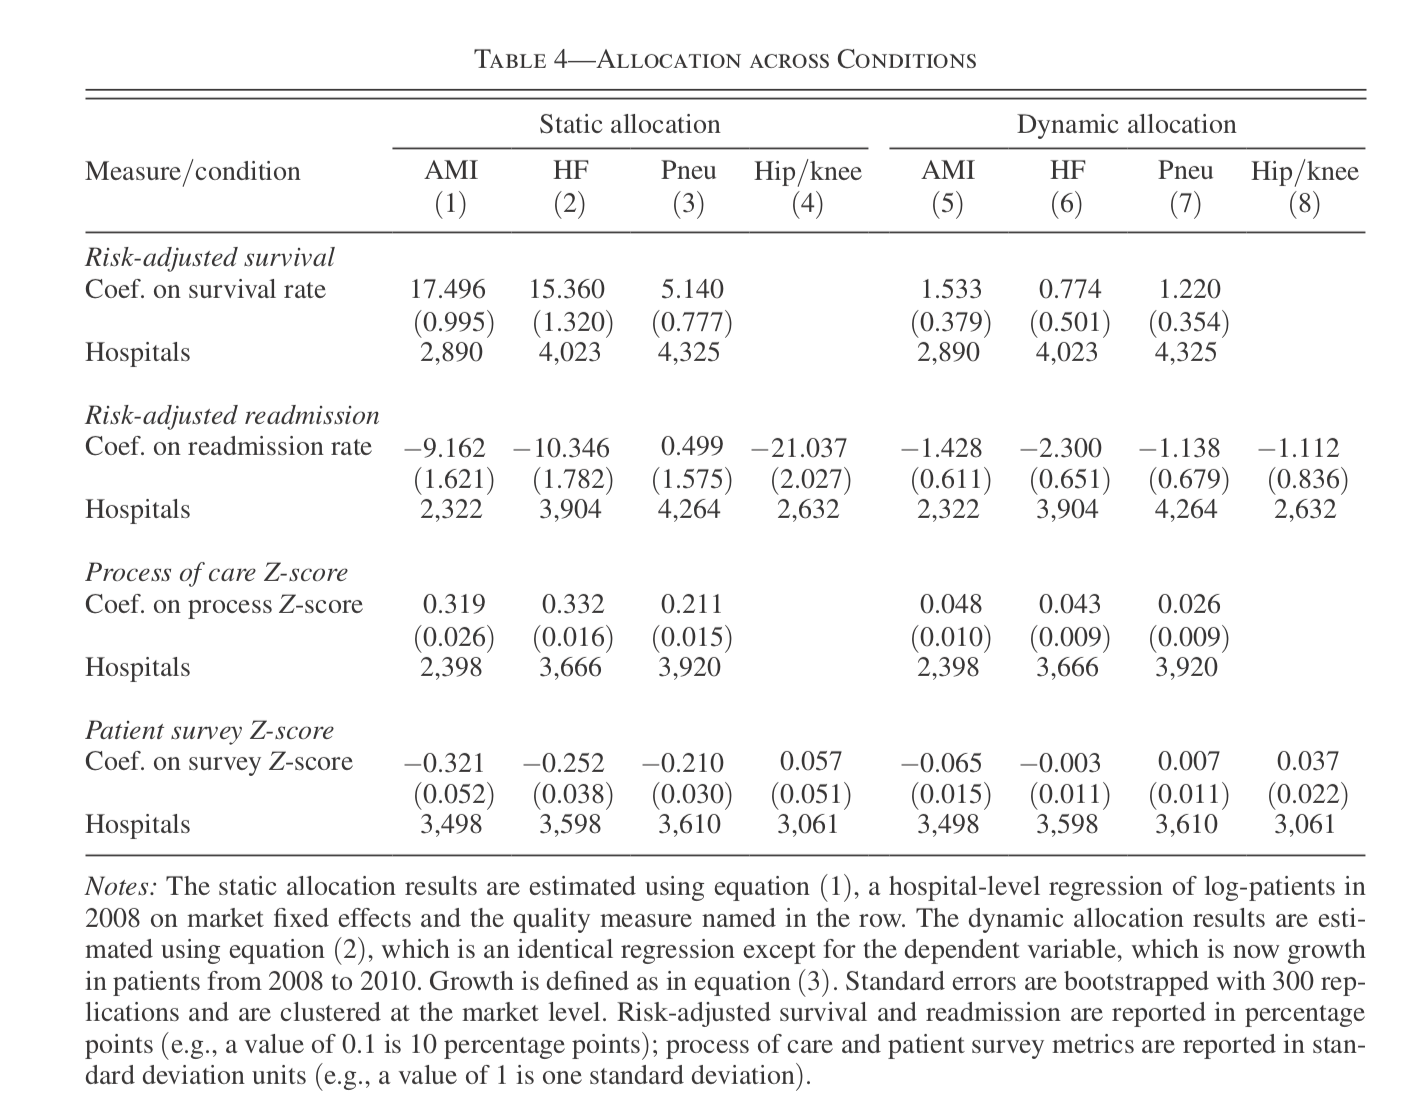
\includegraphics[width=4in]{./resources/hc4.png}
\end{center}
\end{frame}


\begin{frame}{Healthcare Exceptionalism: Production Function}
Hospital Production Function:
\begin{align*}
y_{p}^{s}=a_{h}+\sum_{k} \lambda_{k} r_{p k}+\mu x_{p}+\xi_{p}
\end{align*}
\begin{itemize}
\item $a_h$ is \alert{hospital productivity} (a FE) and variable of interest
\item $y_p$ is a patient outcome (survival-days, etc.)
\item $x_p$ are (log) hospital inputs
\item $r_{pk}$ are patient risk factors.
\item This has interpretation as a \alert{production function}. Why?
\end{itemize}
\end{frame}


\begin{frame}{Healthcare Exceptionalism}
\begin{center}
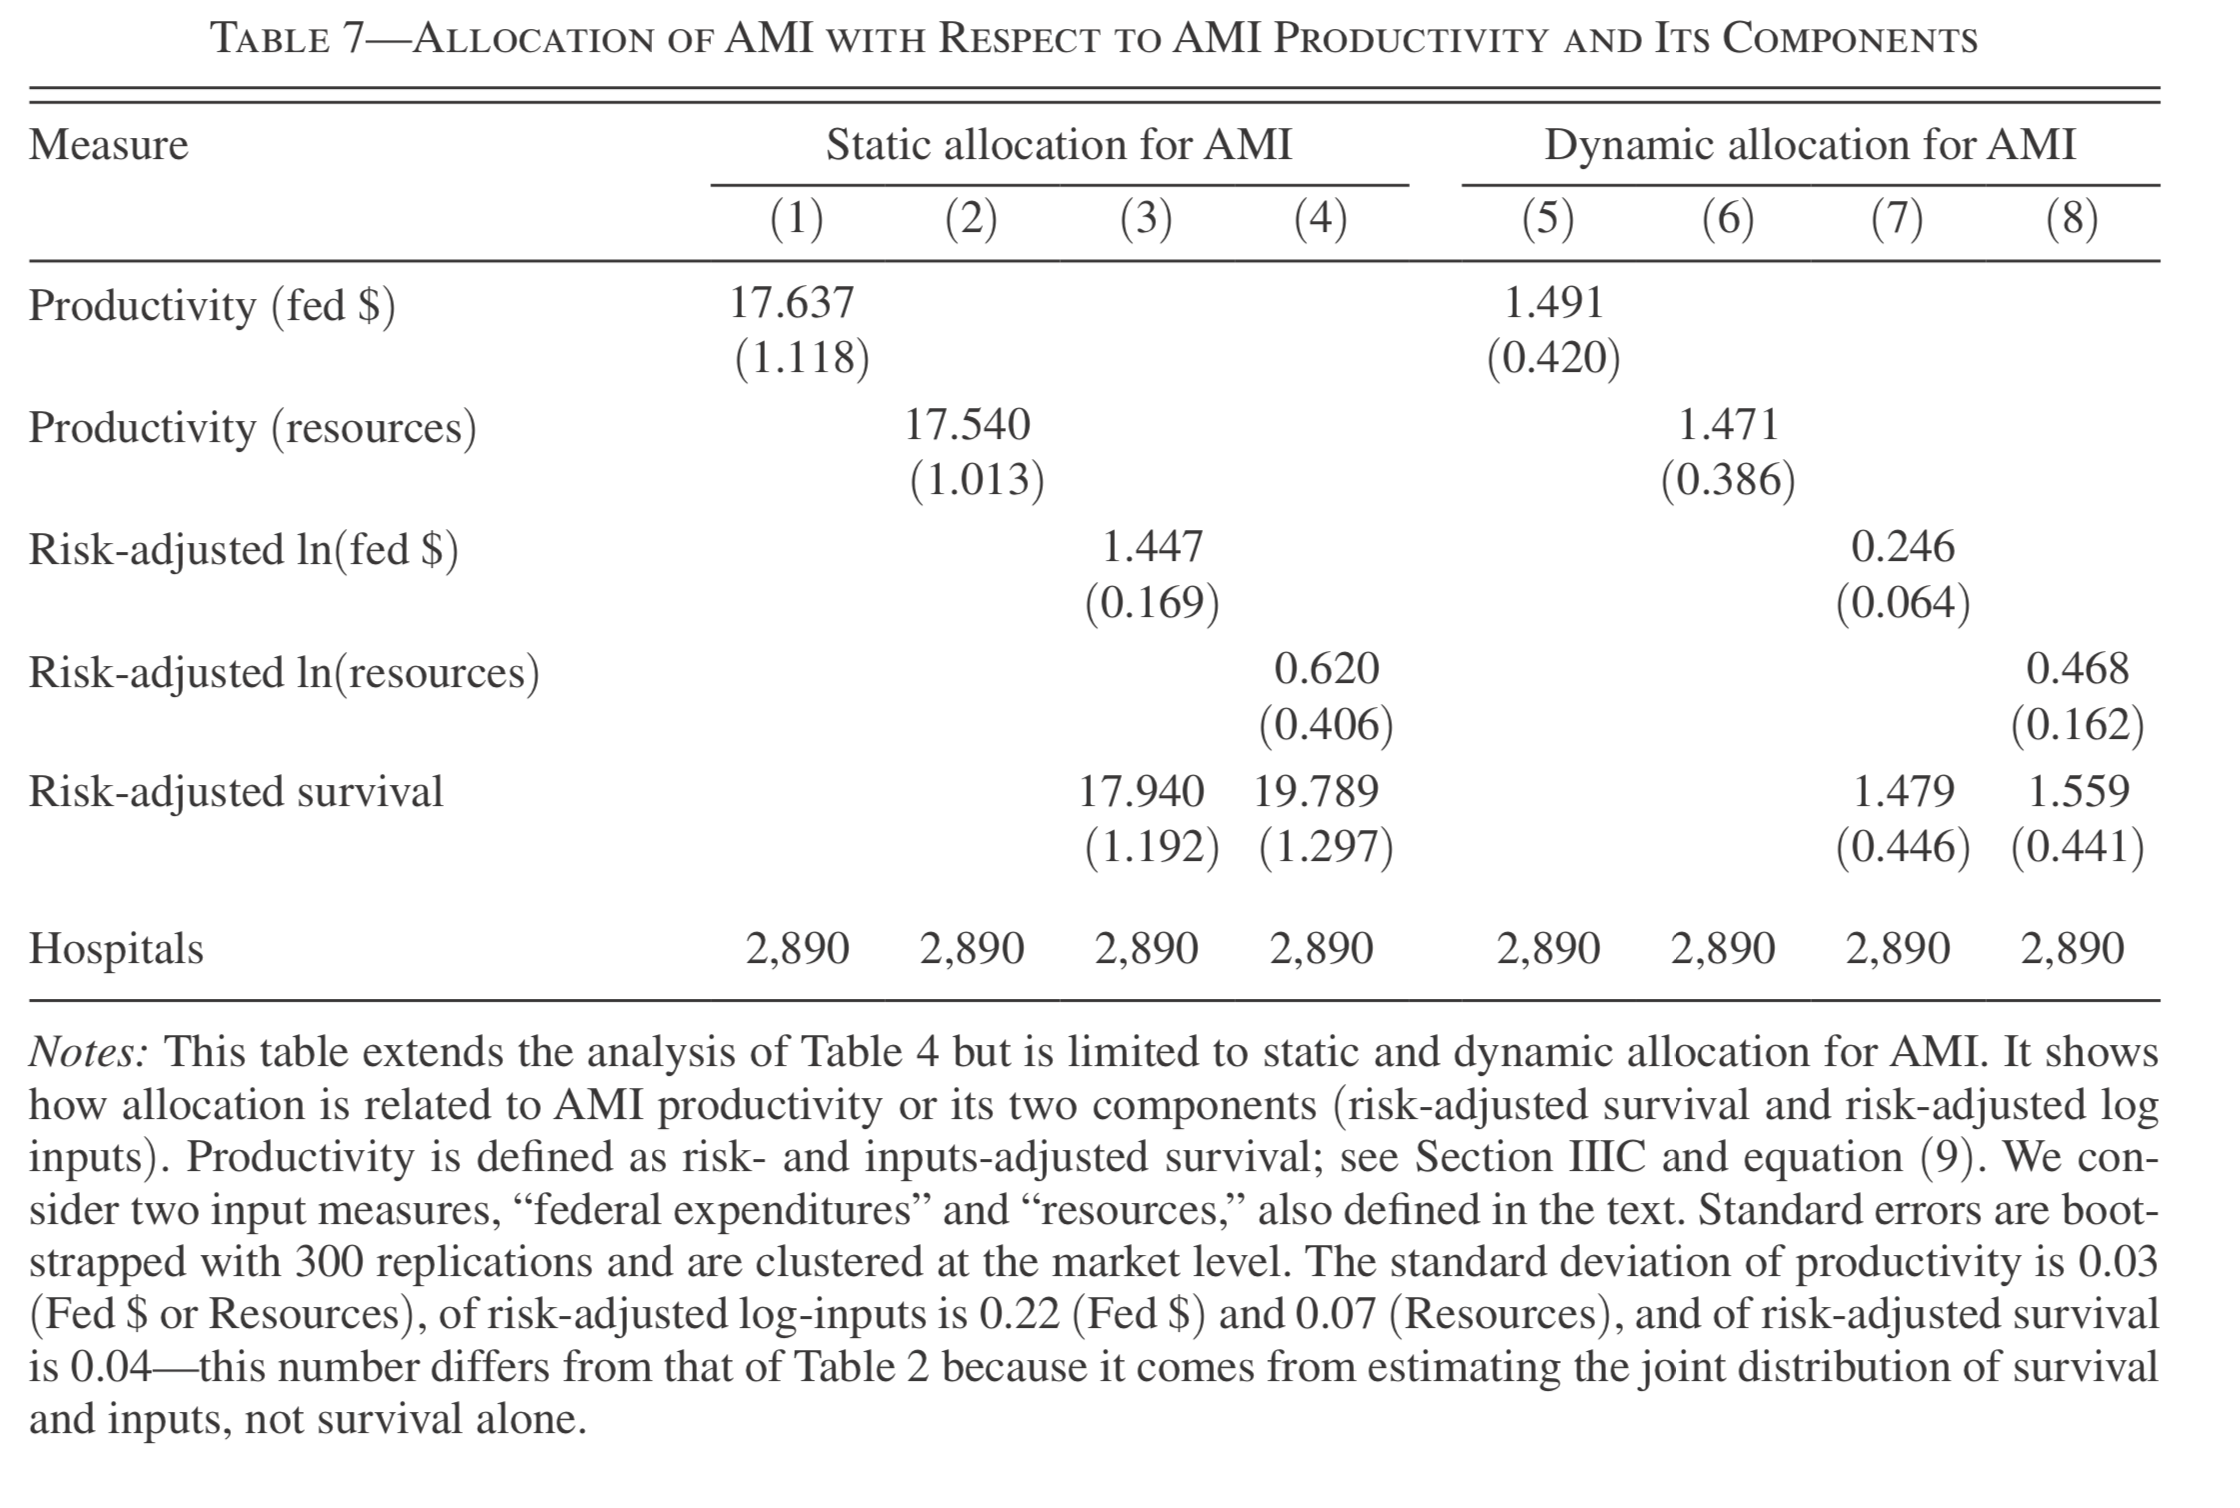
\includegraphics[width=4in]{./resources/hc7.png}
\end{center}
\end{frame}

\begin{frame}{Healthcare Exceptionalism: EB Adjustment}
\begin{center}
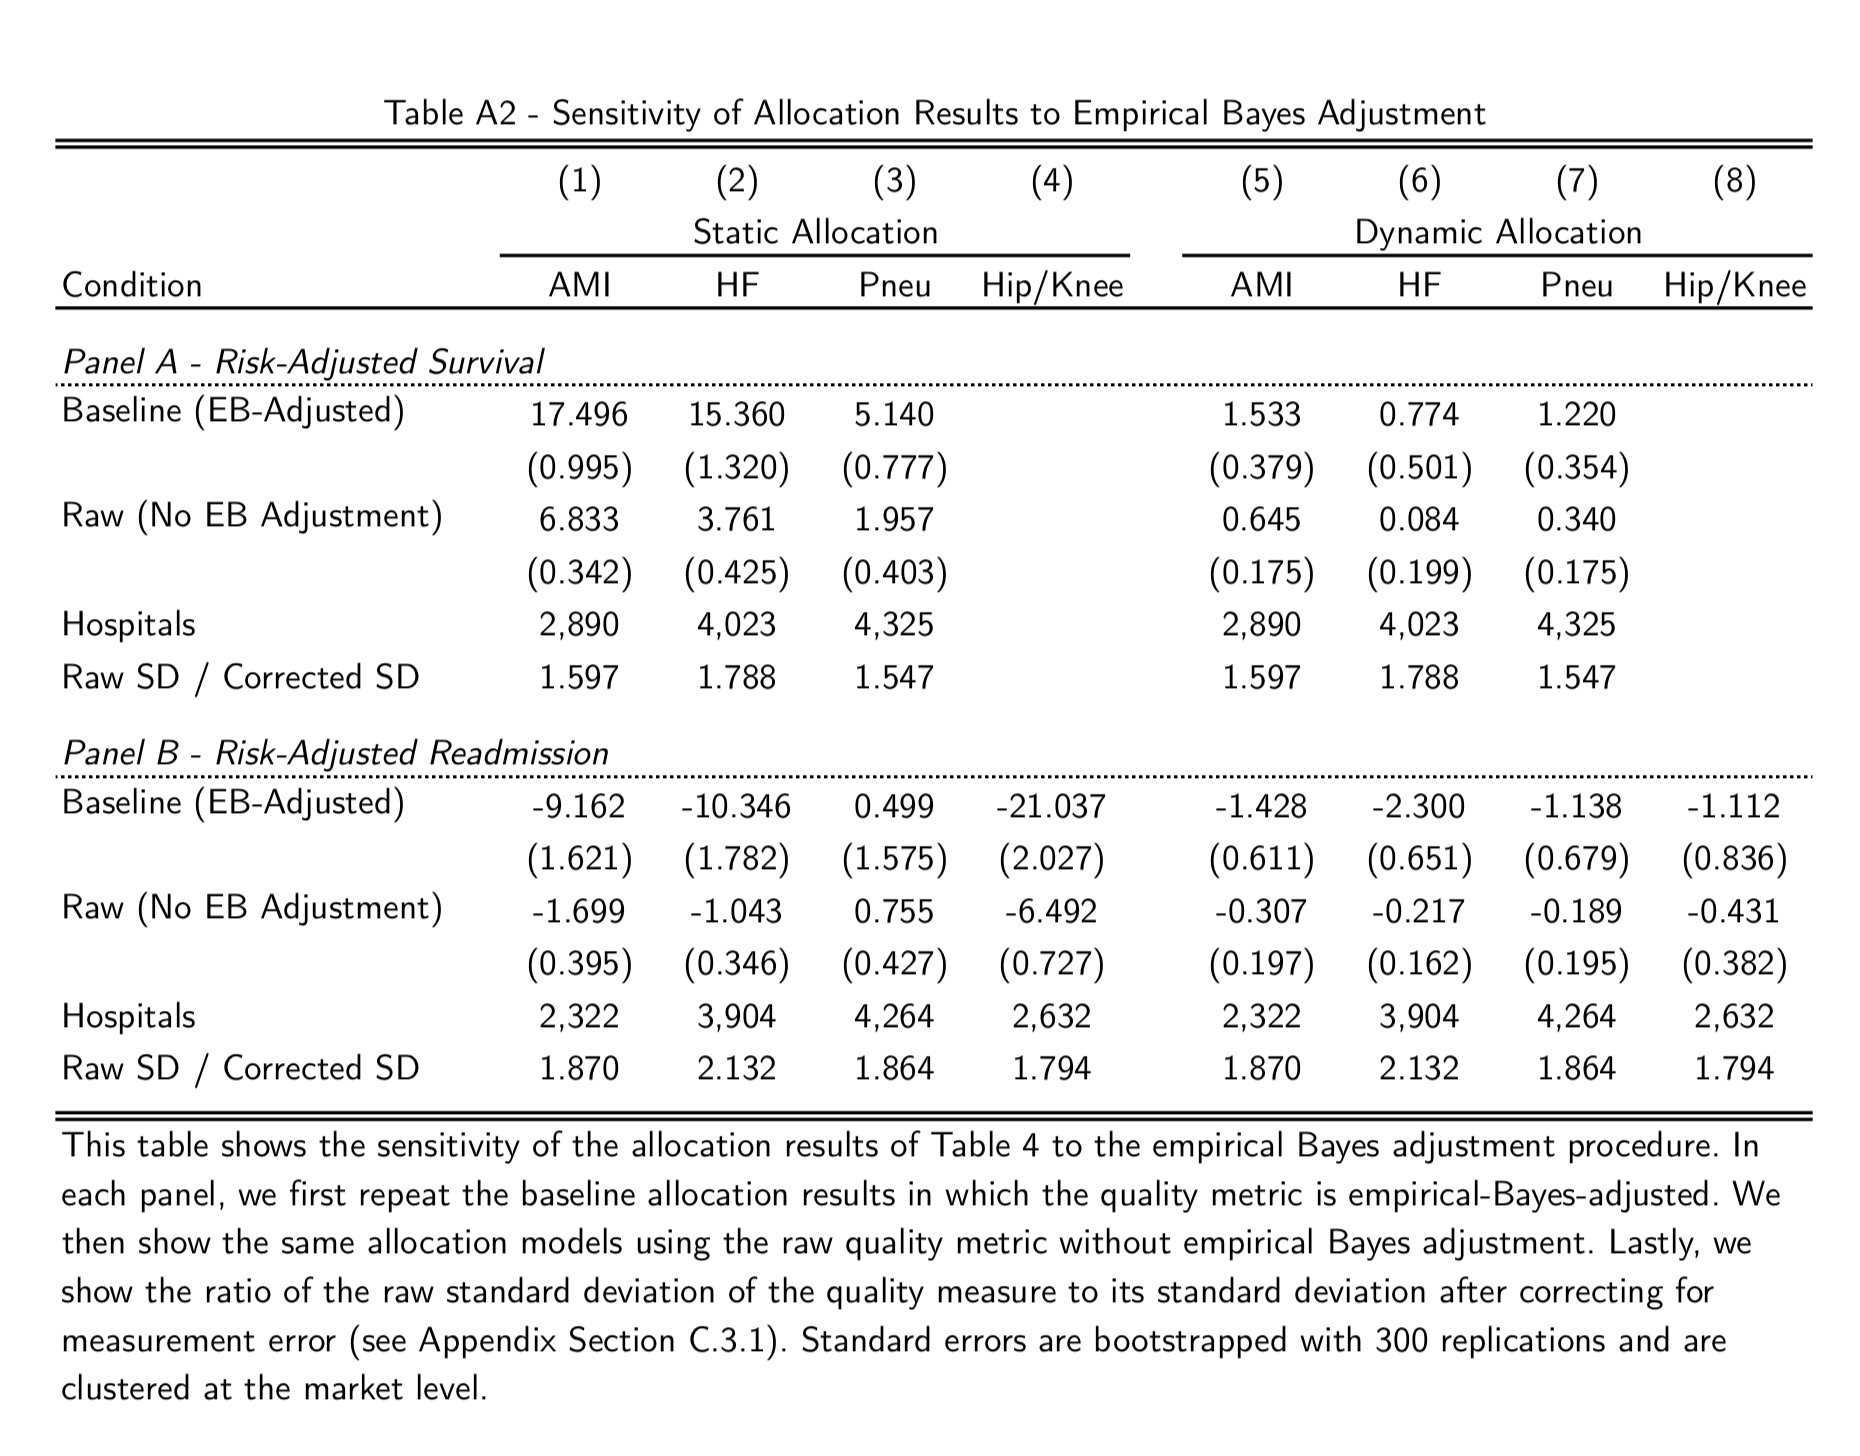
\includegraphics[width=4in]{./resources/hc_a2.png}
\end{center}
\end{frame}



\section{Empirical Bayes}
\begin{frame}{What is Emprical Bayes?}
\begin{itemize}
\item Priors can be an important modeling choice
\item But what makes a good prior?
\begin{itemize}
\item Sufficiently diffuse
\item As non-informative as possible
\item Don't tip the scales
\item Don't rule out the truth
\end{itemize}
\item Idea: can we use the data itself to construct a prior?
\begin{itemize}
\item If everything is a function of data, are we back in frequentist paradigm?
\item Can we get benefits of Bayes estimation without unpalatable assumptions?
\end{itemize}
\end{itemize}
\end{frame}


\begin{frame}[fragile]{A (famous) Baseball Example}
Suppose we want to estimate batting averages $(AVG)$ for some baseball players
\begin{itemize}
\item $AVG = \frac{\# \text{hits}}{ \# At Bats}$
\item Use data on the first $n=45$ at bats and hits $x_i$ for the 1970 season.
\item Predict the batting average $\mu_i$ for the end of the season  ($n=400-500$ at bats).
\item Obvious estimate is batting average after 45 at bats: $\widehat{\mu}_i^{MLE}= x_i/45$.
\item Is there a better estimate?
\end{itemize}
\end{frame}


\begin{frame}[fragile]{A Baseball Example}
\begin{center}
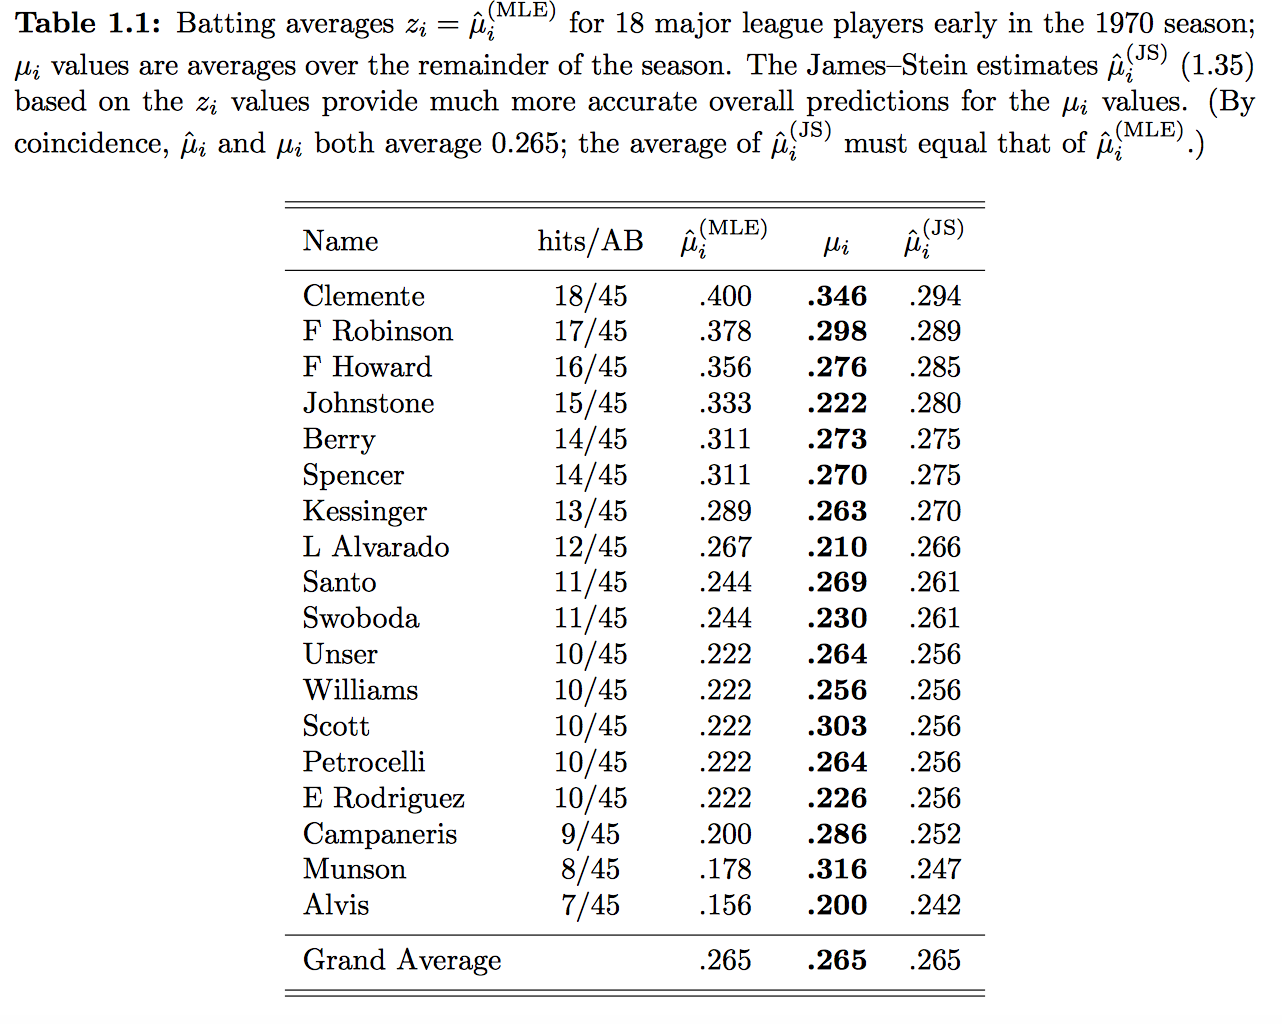
\includegraphics[width=3.5in]{./resources/baseball.png}
\end{center}
\end{frame}

\begin{frame}[fragile]{A (famous) Baseball Example}
Probably we can do better than the MLE here:
\begin{itemize}
\item Thurman Munson wins Rookie of the Year and ends up batting $\mu_i = .316$. If he batted .178 all year, his career would not have lasted long.
\item Clemente's $.400$ seems unlikely to hold up. Last player to hit $> .400$ was Ted Williams $.406$ in 1941.
\item But how?
\end{itemize}
\end{frame}

\begin{frame}[fragile]{Bayesian Shrinkage}
Idea is to take an average between the observed average $y_i$ and the overall mean $\overline{y}$:
\begin{align*}
\widehat{\mu}_i^{JS} &=  (1-\lambda) \cdot \overline{y}  + \lambda \cdot y_i, \quad
\lambda = 1 - \frac{(k-3) \sigma^2}{\sum_i( y_i - \overline{y})^2}
\end{align*}
\begin{itemize}
\item This has the effect of \alert{shrinking} $y_i$ towards the \alert{prior mean} $\overline{y}$.
\item In this case the \alert{prior mean} is just $\overline{y}$ the grand-mean of all players
\item How can information about unrelated players inform us about $\mu_i$?
\item Also consider proportion of foreign cars in Chicago as an additional $y_i$, can this help too?
\item The \alert{shrinkage factor} $\lambda$ depends on sample size and variance, but how is it chosen?
\end{itemize}
\end{frame}



\begin{frame}[fragile]{A Baseball Example}
\begin{center}
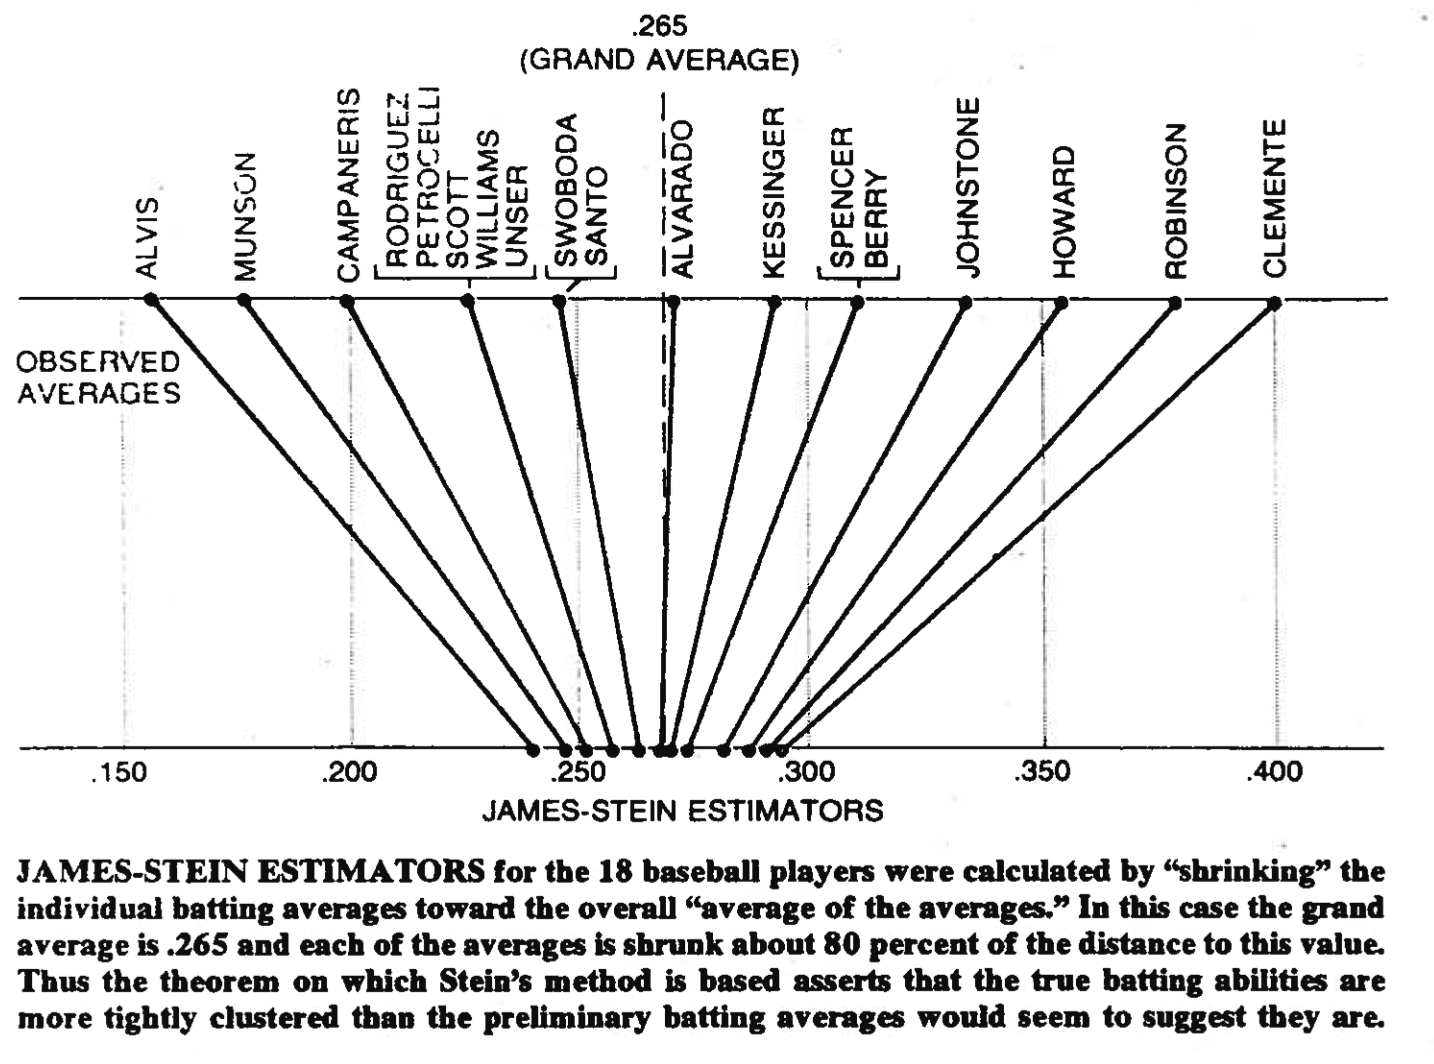
\includegraphics[width=3.5in]{./resources/baseball2.png}
\end{center}
\end{frame}

\section*{Thanks!}




\end{document}